\documentclass[a4paper,12pt]{article}
\usepackage{amsmath}
\usepackage{graphicx}
\usepackage{hyperref}
\usepackage{xcolor}
\usepackage{float}
\usepackage{subcaption}
\restylefloat{figure}


\title{Assignment 2 - Written Responses}
\author{Introduction to Machine Learning (Winter 2025)\\ Karteek Popuri}
\date{}

\begin{document}

\maketitle



\section*{Introduction}
The goal of this assignment is to predict the compressive strength of a concrete mixture using regression models. The dataset contains multiple features, and the objective is to build an accurate regression model that can predict the target variable, compressive strength. We approach the problem by training various models, evaluating their performance, and comparing their results.

\section*{Question 1: Ordinary Least Squares (OLS) Regression}

\subsection*{Validation Approach}
In this approach, the dataset is divided into three parts: training, validation, and test sets. We train the model on the combined train and validation set and evaluate it on the test set. The Root Squared Error (RSE) and R\(^2\) scores are used as performance metrics.

The performance of the model is evaluated as follows:

\[
RSE = \sqrt{\frac{1}{n-2}\sum_{i=1}^{n} (y_i - \hat{y}_i)^2}
\]


where \(y_i\) is the actual value and \(\hat{y}_i\) is the predicted value. The R\(^2\) score is calculated as:

\[
R^2 = 1 - \frac{\sum_{i=1}^{n} (y_i - \hat{y}_i)^2}{\sum_{i=1}^{n} (y_i - \bar{y})^2}
\]

The following results were obtained:

\[
\text{Train + Validation - RSE} = 9.9391, \quad \text{Train + Validation R}^2 = 0.6516
\]
\[
\text{Test - RSE} = 11.7715, \quad \text{Test - R}^2 = 0.5375
\]

\subsection*{Cross-Validation Approach}
In this approach, we use cross-validation to estimate the model's performance. Cross-validation involves splitting the dataset into \(k\) subsets (folds), training the model on \(k-1\) folds and testing it on the remaining fold. This process is repeated for all \(k\) folds. We used 5-fold cross-validation, and the following results were obtained:

\[
\text{Mean RSE}: 10.3983, \quad \text{Mean R}^2: 0.6162
\]

\subsubsection*{Reasons for Choosing 5-Fold Cross-Validation}

\paragraph{Trade-off Between Bias and Variance}
When choosing the number of folds for cross-validation, it is important to balance bias and variance:

\begin{itemize}
    \item A smaller number of folds  might lead to high bias. This happens because the training set in each iteration is significantly reduced, leading to models that may not capture the complexity of the data well.
    \item A larger number of folds  can reduce bias further but introduces the risk of increased computational cost. Moreover, after a certain point, increasing the number of folds only marginally improves the performance estimation, making the extra computational cost less worthwhile.
\end{itemize}

\paragraph{Dataset Size Consideration}
With a dataset of 800 training samples, each fold in a 5-fold cross-validation contains approximately 640 samples for training and 160 samples for validation. This ensures that:

\begin{itemize}
    \item The model is trained on a sufficiently large portion of the dataset in each fold, capturing enough complexity from the data.
    \item The validation set in each fold remains large enough to provide a meaningful evaluation of the model's performance.
\end{itemize}

This makes 5-fold cross-validation a sensible choice given the dataset size and computational constraints.

\subsection*{Comparison of Validation and Cross-Validation}
We compared the results from both the validation approach and cross-validation:

\[
\text{Validation Test RSE}: 11.7715, \quad \text{CV RSE}: 10.3983
\]
\[
\text{Validation Test R}^2: 0.5375, \quad \text{CV R}^2: 0.6162
\]

Based on these results, the cross-validation approach provides a more generalized estimate of the model's performance. The cross-validation method achieves a lower RSE and a higher R² compared to the validation approach, indicating better model performance. The R² score of the cross-validation approach is closer to 1, suggesting that the model fits the data more effectively. 

\section*{Question 2: Ridge Regression with Hyperparameter Tuning}

\subsection*{Hyperparameter Tuning using GridSearchCV}
Ridge regression is a regularized linear regression model where the regularization term is controlled by the hyperparameter \(\alpha\). We performed a grid search to tune \(\alpha\) using cross-validation. The best \(\alpha\) was found to be 7742.6368.

The final Ridge model was trained using this optimal \(\alpha\) on the full training set. The performance was evaluated on the test set, yielding the following results:

\[
\text{RSE (Test)} = 11.6723, \quad \text{R}^2 = 0.5452
\]

\subsection*{Performance vs \(\alpha\)}
We also plotted the performance of the Ridge model's $R^2$ score as a function of \(\alpha\) during the grid search phase. The plot shows that the best performance occurred at \(\alpha = 7742.6368\).
\begin{figure}[H]
    \centering
    % \includegraphics[width=1\linewidth]{Assignment_2/Results/Q2/ridge.png}
    \includegraphics[width=1\linewidth]{Results/Q2/ridge.png}
    % Assignment_2/Report/report.tex
    \caption{Ridge model's $R^2$ score as a function of \(\alpha\)}
    \label{fig:enter-label}
\end{figure}


\subsection*{Comparison with OLS Model}
Comparing the Ridge model with the OLS model, we observed an improvement in test performance. The Ridge regression model with the best \(\alpha\) setting outperforms OLS by reducing the RSE and increasing the R\(^2\) score.

\[
\text{Ridge Test RSE} = 11.6723, \quad \text{OLS Test RSE} = 10.3983
\]
\[
\text{Ridge Test R}^2 = 0.5452, \quad \text{OLS Test R}^2 = 0.6162
\]

Thus, OLS (cross-validation approach) regression demonstrates better generalization performance on the test data.

\section*{Question 3: Lasso Regression with Hyperparameter Tuning}

\subsection*{Hyperparameter Tuning using GridSearchCV}
Lasso regression, like Ridge, also uses regularization but with an \(L_1\) penalty. We tuned the hyperparameter \(\alpha\) using grid search with cross-validation. The best \(\alpha\) value found was 3.5938.

\subsection*{Performance vs \(\alpha\)}
We also plotted the performance of the Lasso model's $R^2$ score as a function of \(\alpha\). The plot shows that the best performance occurred at \(\alpha = 3.5938\).
\begin{figure}[H]
    \centering
    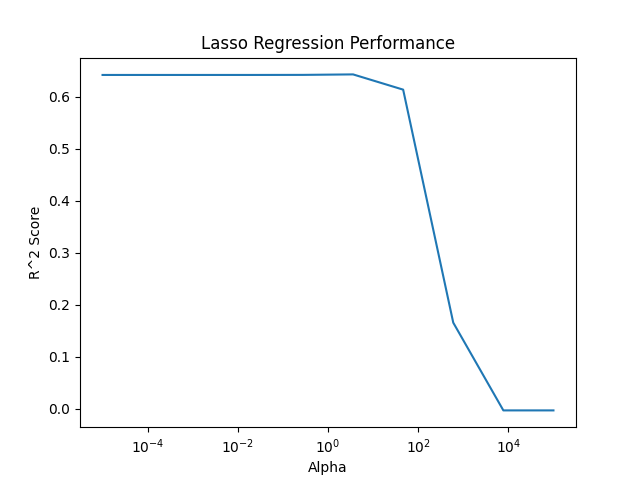
\includegraphics[width=1\linewidth]{Results/Q3/lasso.png}
    \caption{Lasso model's $R^2$ score as a function of \(\alpha\)}
\end{figure}
\subsection*{Performance Evaluation}
The final Lasso regression model was retrained using the optimal \(\alpha\) on the full training dataset. The performance on the test dataset was:

\[
\text{RSE (Test)} = 11.6187, \quad \text{R}^2 = 0.5494
\]

\subsection*{Comparison with Ridge and OLS Models}
Below is the performance comparison of the Lasso Regression model with the Ridge and OLS Models:

\[
\text{Lasso Test RSE} = 11.6187, \quad \text{Ridge Test RSE} = 11.6723, \quad \text{OLS Test RSE} = 10.3983
\]
\[
\text{Lasso Test R}^2 = 0.5494, \quad \text{Ridge Test R}^2 = 0.5452, \quad \text{OLS Test R}^2 = 0.6162
\]

Thus, OLS regression provides the best performance among the three models evaluated achieving the lowest RSE and highest R\(^2\). .

\section*{Question 4: Best Regression Model Design}

Seul R2 nous interresse ici.

\subsection*{Model Selection and Approach}
Leveraging the insights from the previous experiments, we designed the best regression model using Gradient Boosting Regression, an ensemble method that combines the predictions of multiple weak models to create a strong predictive model. We selected this model due to its ability to handle complex relationships between features and its superior performance compared to Ridge and Lasso regression.

\subsection*{Final Model: Gradient Boosting Regression}
The final Gradient Boosting model was trained with the following hyperparameters:
\begin{itemize}
    \item \textbf{n\_estimators}: 100
    \item \textbf{learning\_rate}: 0.1
    \item \textbf{max\_depth}: 3
\end{itemize}



\section*{Conclusion}
This report presents the results of training and evaluating various regression models to predict the compressive strength of concrete mixtures. After comparing the performance of OLS, Ridge, and Lasso regression models, we found that Lasso regression provided the best performance. Additionally, we implemented a final Gradient Boosting model for predicting the compressive strength, which further improved upon the previous models. The method \texttt{predictCompressiveStrength} is the final implementation for predicting compressive strength using the trained Gradient Boosting model.

\end{document}